\vspace{1cm}
\subsubsection{Căutarea celei mai bune mutări}
\vspace{1cm}

Șahul este un joc cu suma nulă, adică câștigul unui jucător este perfect echilibrat de
pierderea celuilalt (dacă o mutare îi oferă unui jucător scorul de 200, pentru oponent
mutarea va avea scorul -200), ceea ce permite folosirea unui algoritm de căutare
numic \textit{Negamax}.

Algoritmul constă în generarea unui arbore în care muchiile reprezintă câte o mutare legală,
iar nodurile pozițiile după efectuarea mutărilor din rădăcină până la nod până la o adâncime
fixă. Acest arbore se parcurge într-un mod similar cu algoritmul DFS, iar fiecărui nod i se
atribuie un scor egal cu:
\begin{itemize}
	\item Rezultatul funcției de evaluare, dacă nodul este o frunză
	\item Maximul dintre scorurile descendențiilor, cu semn opus (deoarece o mutare bună pentru
	      oponent este o pierdere pentru jucătorul curent), dacă nodul nu este o frunză
\end{itemize}
La final vom ști din rădăcină ce mutare este optimă pentru jucătorul curent.

\vspace{1cm}
În mod general, acest algoritm se implementează astfel:
\begin{lstlisting}[language=RustHtml]
int negaMax( int depth ) {
    if ( depth == 0 ) return evaluate();
    int max = -INF;
    for ( all moves)  {
        score = -negaMax( depth - 1 );
        if( score > max )
            max = score;
    }
    return max;
}
\end{lstlisting}
\vspace{1cm}

În practică acest algoritm este foarte ineficient deoarece caută un număr foarte mare de noduri,
și se poate optimiza prin nenumărate moduri. Funcția de căutare folosește următoarele optimizări:
\begin{itemize}
	\item Alpha-beta pruning
	\item Tabele de transpoziții
	\item Move ordering
	\item Iterative deepening
	\item Principal Variation
\end{itemize}

De asemena, pentru șah nu este de ajuns căutarea până la o adâncime fixă, trebuie continuată
căutarea până la poziții unde nu există mutări care capturează piese.

De exemplu, în cazul în care căutarea ar ajune în poziția de mai jos și se mai poate evalua
o singură mutare în adâncime, mutarea regină la b6 ar fi considerată o mutare foarte bună
deoarece capturează un nebun, însă la următoarea mutare regina poate fi capturată de pionul de
la a7. Această îmbunătățire se numește \textit{quiescence search}.

\vspace{1cm}
\begin{center}
	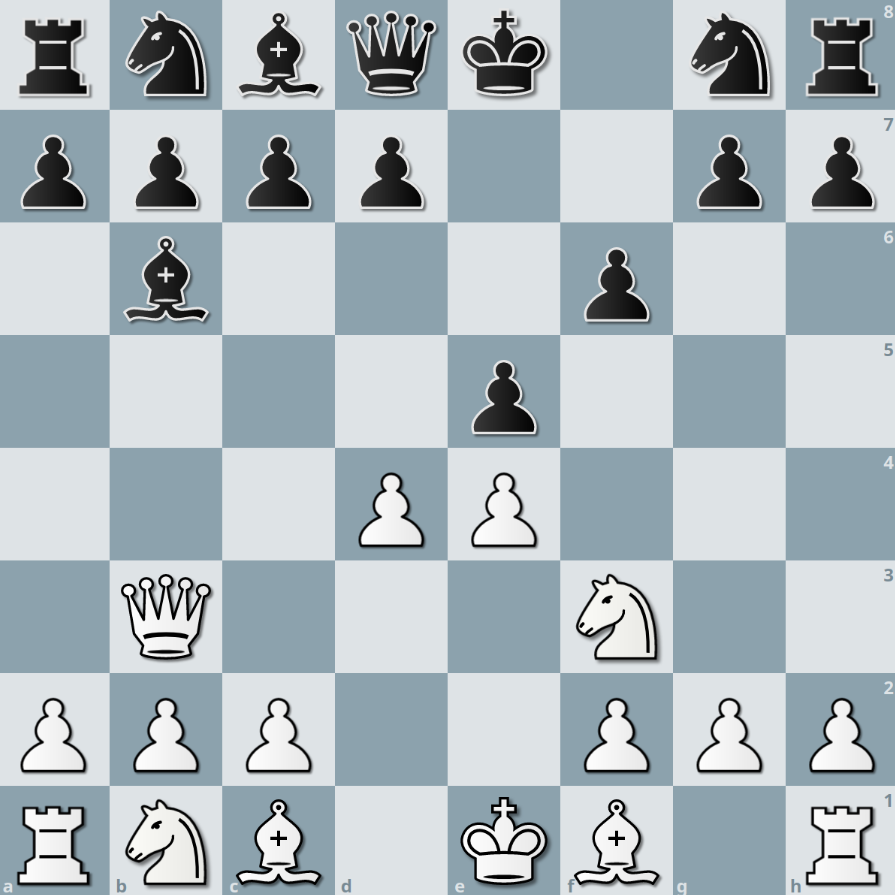
\includegraphics[width=10cm]{3/alg/quiescence.png}
\end{center}
\vspace{1cm}

\vspace{1cm}
\paragraph{Alpha-beta pruning}\mbox{} \\

Această optimizare este cea mai importantă și cea care permite implementarea tuturor restul
optimizărilor și constă în adăugarea a 2 parametrii alpha și beta care reprezită scorul minim
pe care jucătorul curent îl poate obține, repsectiv scorul maxim pe care oponentul îl poate
obține. Folosind aceste 2 numere se pot reduce semnificativ numărul de noduri căutate, dar
obținând garantat același rezultat.

După ce se calculează scorul unei mutări posibile se verifică dacă este mai mare sau egal
decât beta. Dacă da atunci nu mai are sens căutarea acestui nod deoarece oponentul poate să facă
o mutare care garantează un scor mai mare sau egal decât orice orice altă mutare găsită până acum,
deci este o mutare proastă pentru jucătorul curent și se returnează beta.

\vspace{1.5cm}
Implementarea generală este asemănătoare cu cea de la \textit{negamax}:
\begin{lstlisting}[language=RustHtml]
int negaMax(int depth, int alpha, int beta) {
    if (depth == 0) return evaluate();
    for (all moves)  {
        score = -negaMax(-beta, -alpha, depth-1);
        if (score >= beta) {
            return beta;
        }
        if (score >= alpha) {
            alpha = score;
        }
    }
    return alpha;
}
\end{lstlisting}

\vspace{1cm}
\paragraph{Move ordering}\mbox{} \\

Optimizarea precedentă funcționează mai bine atunci când găsește o mutare bună mai repede,
astfel se pot ordona mutările înainte de a fi parcurse. Ordonarea se poate face atribuind fiecărei
mutări un scor general și apoi sortarea în ordine descrescătoare după scor.

O metodă simplă de atribuire a scorului general este
\begin{itemize}
	\item Dacă mutarea este o captură: 10 * p2 - p1, unde p1 este valoarea piesei cu care se
	      capturează și p2 este valoarea piesei capturată
	\item 0, în caz contrar
\end{itemize}
\vspace{0.5cm}
De exemplu dacă avem mutările:
\begin{itemize}
	\item Capturarea unei ture cu un cal
	\item Mutarea unui cal pe un spațiu gol
	\item Capturarea unei ture cu un pion
\end{itemize}
După sortare se vor căuta în ordinea:
\begin{itemize}
	\item Capturarea unei ture cu un pion
	\item Capturarea unei ture cu un cal
	\item Mutarea unui cal pe un spațiu gol
\end{itemize}

\vspace{1cm}
\paragraph{Iterative deepening și principal variation}\mbox{} \\

Iterative deepening este o tehnică de a gestiona timpul în care algoritmul găsește o mutare
și constă în rularea căutarea de mai multe ori, începând de la adâncimea maximă 1 până la
limita fixată, iar după fiecare căutare completă, dacă a trecut timpul alocat găsirii acestei
mutări se ignoră rezultatul curent și se returnează cel precedent. (Pentru a opri căutarea
curentă la timp se verifică periodic în funcția de \textit{negamax} dacă a trecut timpul).

Doar această tehnică nu este o optimizare, ci din potrivă se caută aceleași noduri de mai multe
ori. Optimizarea se face prin tehnica \textit{principal variation} care constă în căutarea
mutărilor care au dus la cel mai bun scor iterația trecută înaintea tuturor celorlate mutări
(acestor mutări li se atribuie un scor mai mare decât celorlalte în funcția de sortare),
deoarece cea mai bună mutare în căutarea până la adâncimea k este probabil o mutare bună
și la căutarea k+1.

\vspace{1cm}
\paragraph{Tabele de transpoziții}\mbox{} \\

Să considerăm poziția de mai jos. Există 4 serii distincte de mutări prin care se poate ajunge
în acest punct (numite transpoziții) și după fiecare se vor evalua aceleași mutări,
ceea ce este ineficient.

Astfel după ce am evaluat o poziție se memorează într-un tabel (reprezentat printr-un vector mare)
adâncimea la care s-a făcut evaluarea, scorul rezultat și punctul din funcția de \textit{alpha-beta}
unde s-a memorat rezultatul (în if-ul cu beta, în if-ul cu alpha sau la final)

Acum, în funcția de \textit{alpha-beta} înainte de for se verifică dacă în tabelul de transpoziții
există o intrare cu poziția dată cu adâncimea mai mare sau egală decât adâncimea curentă și
care să satisfacă limitele impuse de alpha și beta din căutarea curentă. În cazul în care există
se returnează scorul ținut minte în tabel, altfel se continuă cu căutarea normală.

Pentru memorarea unei poziții într-un array trebuie generat un index aproape unic folosind
\textit{hashuri Zobrist} care funcționează astfel:
\begin{itemize}
	\item Se generează mai multe numere la întâmplare (pe 64 de biți) care rămân aceleași
	      pe parcusul căutării
	      \begin{itemize}
		      \item Câte 12 pentru fiecare tip de piesă pentru fiecare pătrat (720 de numere)
		      \item 16 numere pentru fiecare stare de rocadă (sunt 4 rocade, deci $2^4$ numere)
		      \item 8 numere pentru fiecare coloană pe care se poate face mutarea en passant
		      \item 1 număr pentru culoarea jucătorului
	      \end{itemize}

	\item Transformarea unei poziții într-un index se face astfel:
	      \begin{enumerate}
		      \item Începem cu indexul egal cu 0
		      \item Pentru fiecare piesă de pe tablă se face xor între index și numărul generat
		            pentru piesă și poziția ei pe tablă
		      \item Se face xor între index și starea de rocadă
		      \item Dacă se poate juca en passant, se face xor între index și coloană
		      \item Dacă jucătorul curent are piesele cu culoarea neagră se face xor între index
		            și numărul pentru culoare
		      \item Se returnează indexul obținut
	      \end{enumerate}
\end{itemize}

Indexul rezultat va fi un număr pe 64 de biți, posibil foarte mare, și nu poate fi folosit
direct ca index, astfel tabelul de transpoziții va avea o mărime fixă, iar indexul in tabel
se va calcula prin indexul generat modulo mărimea tabelului.
